\chapter{Contributions}

In this section we will tie together the different publications made during the course of the PhD studies. We will focus on the general message of the publications in relation to the goal of the PhD. We remand to the full text of the individual publications in Appendices~ \ref{sec:glass}-\ref{sec:vrbrdf} for the full technical details.

\section{Motivation}
(Figure: Fields in which we need instant feedback on appearance: 3d printing, artist feedback, quality control, meat)
Is path tracing good enough?

How can we make interactive appearance prediction

What is photorealistic?

Here cite our preliminary study (Interactive appearance prediction...) as motivation for both photorealism and interactivity.

Achieveing fast techniques for photorealisitic rendering important in various fields.


\section{Defining photorealistic rendering}
\begin{figure}
\begin{tabular}{@{}c@{}c@{}}
	 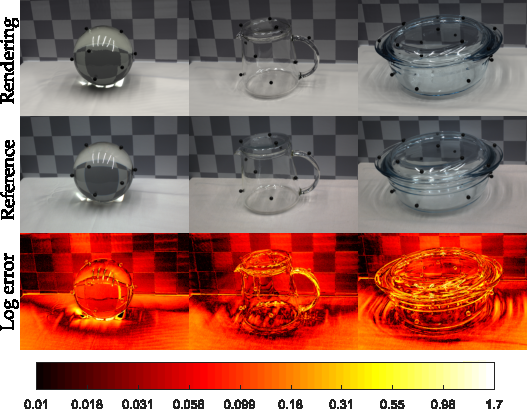
\includegraphics[height=4.3cm]{figures/comparison} & \hspace{2em}
	 \includegraphics[height=4.3cm]{figures/glass_bowl_analysis_by_synthesis}  \\
\end{tabular}
\caption{\fixme{Write me.}} %The red rectangle shows where we estimated RMSE in Table \ref{table:quant}.}
\label{fig:teaser}
\end{figure}


Take home points:
\begin{itemize}
\item Preliminary study: appearance prediction is important, interactivity is important.
\item Realistic reconstruction is hard. 
\item At the moments, it is not possible to evaluate how good path tracing is.
\item Tough, we can evaluate and measure parameters from the scene. Being able to compare is what it is all about.
\item Fine details make the difference, especially in geometry
\item Identify problems in acquisition, rendering and reconstruction, using the dataset to improve current rendering techniques.
\item Publicly available dataset?

\end{itemize}

\section{Interactive rendering of scattering media}
\begin{figure}
\begin{tabular}{@{}c@{}c@{}}
	 \includegraphics[width=0.5\columnwidth]{figures/teaser_render.png} &
	 \includegraphics[width=0.5\columnwidth]{figures/ref_img.jpg}  \\
	rendering & photograph \\
\end{tabular}
\caption{Cloudy apple juice photographed and rendered using our appearance model. In the model, apple particle concentration (0.8 g/l) and apple storage period (4 days) were selected to match the photograph.} %The red rectangle shows where we estimated RMSE in Table \ref{table:quant}.}
\label{fig:teaser}
\end{figure}

\begin{figure}
\begin{tabular}{@{}c@{$\,$}c@{}c@{}c@{}}
& directional dipole, 6 fps & standard dipole and VPLs \\
\begin{sideways}\hspace*{1.5em}our method\end{sideways} &
\includegraphics[width=0.48\columnwidth]{figures/candle_holder_directional_6fps.png} &
\includegraphics[width=0.48\columnwidth]{figures/candle_holder_jensen_converged.png} \\[-4pt]
\begin{sideways}\hspace*{1.7em}ray tracer\end{sideways} &
\includegraphics[width=0.48\columnwidth]{figures/scene_comparison_optix_6fps.png} &
\includegraphics[width=0.48\columnwidth]{figures/scene_comparison_converged.png} \\[-0.5ex]
& directional dipole, 6 fps & directional dipole, reference \\[-1ex]
\end{tabular}
\caption{Equal time comparison (left column) of our method with the reference method and qualitative comparison with diffuse subsurface scattering (upper right) and the converged reference solution (lower right). The scene is lit by a point light in a white grapefruit candle holder.} % Emerging light illuminates a diffuse Stanford Bunny on a tabletop.}
\label{fig:optixcomparison}
\end{figure}

Refer to case study again.

\begin{itemize}
\item cloudy apple juice study.
\item Rouch estimate during production
\item It is possible to apply complicated rendering models (like directional SSS) in an interactive domain
\item Working under constraints
\item Texture-free, deformable model
\item Leveraging the strength of rasterization
\item Multiple lights
\item Global illumination extensions: how you do reuse information that you have already available
\item Maps of scattered radiosity
\item Progressive rendering
\item Interactive transport of emergent light from deformable objects
\item Transport of light behind translucent objects.
\end{itemize}


\section{Interactive stable ray tracing}

\begin{figure}
\begin{tabular}{@{}c@{}c@{}@{}c@{}}
	 \includegraphics[width=0.33\textwidth]{figures/ss_2x_rect_370_300_300_300_frame_211.png} &
		 \includegraphics[width=0.33\textwidth]{figures/ss_2x_taa_rect_370_300_300_300_frame_211.png} &
		  \includegraphics[width=0.33\textwidth]{figures/ss_32x_rect_370_300_300_300_frame_211.png} \\	 
Supersampling, 2 spp & Supersampling, 2 spp 	& Supersampling, 32 spp \\
  					 & + temporal antialiasing 	&  \\
sharpness: 0.7924 & sharpness: 0.5348 & sharpness: 0.6771  \\
	 \includegraphics[width=0.33\textwidth]{figures/srt_1_rect_370_300_300_300_frame_211.png} &
	 	 \includegraphics[width=0.33\textwidth]{figures/srt_1_ti_rect_370_300_300_300_frame_211.png} &
	  \includegraphics[width=0.33\textwidth]{figures/ss_32x_rect_370_300_300_300_frame_211.png}
 \\
Stable ray tracing, 1 spp & Stable ray tracing, 1 spp & Supersampling, 32 spp \\
 & + temporal integration &  \\
sharpness: 0.7085 & sharpness: 0.6060 & sharpness: 0.6771 \\[-1.5ex]
\end{tabular}
\caption{Including indirect illumination, the different techniques are here applied to a frame in the Sponza video.}
\label{fig:sponza_video_frame}
\end{figure}


\begin{itemize}
\item Take home message: recycling information can be useful to improbe temporal stability 
\item Leveraging ray tracing strengths against rasterization
\item Reprojection 
\item Sharp and antialiased
\item Application to photorealistic rendering in the form of indirect global illumination
\item Foundation technique to combine with existing ones
\item Spatial aliasing
\item Good results with progressive path tracing.
\end{itemize}

\section{Applying interactive photorealistic techniques}
\begin{figure}
\centering
\begin{tabular}{@{}c@{}c@{}}
	 \includegraphics[height = 4.3cm]{figures/screen1_crop} &
		 \includegraphics[height = 4.3cm]{figures/person} \\[-2.5ex]
\end{tabular}
  \caption{Pictures illustrating our VR demo application, with an in-game screenshot (left) and a picture of the setup (right). }
  \label{fig:teaser}
\end{figure}

\begin{itemize}
\item Application to photorealisitic rendering to hard real time constratins
\item Hint at future work that can be done
\item Practical purpose: debug acquired BSRDF models.
\item Apply real time techniques
\item More constraints.
\end{itemize}

\section{Discussion}